\documentclass{beamer}

\mode<presentation>

\usetheme{Pittsburgh}


\usepackage[utf8]{inputenc}
\usepackage{ beamerthemesplit}
\usepackage{caption}
\usepackage{adjustbox}
\newtheorem*{teor}{Teorema}
\newtheorem*{teort}{Teorema de Tibor Radó}
\newtheorem*{lema}{Lema}
\newtheorem*{ejem}{Ejemplos}
\newtheorem*{prop}{Proposición}
\newtheorem*{defi}{Definición}

\newcommand{\specialcell}[2][c]{%
	\begin{tabular}[#1]{@{}c@{}}#2\end{tabular}}


%\mode<handout>
{
\beamertemplatesolidbackgroundcolor{black!5}
}
\usepackage{amssymb,amsmath,amsfonts,graphicx,float,epsfig,enumerate}
\usepackage{subfigure}
\usepackage{amsopn}
\usepackage{fancyhdr}
\renewcommand{\figurename}{}

\renewcommand{\baselinestretch}{1}

% \newenvironment{flushenum}{
% \begin{enumerate}
%   \setlength{\leftmargin}{0pt}
% }{\end{enumerate}}

\sloppy

\parindent 0pt

%\usepackage[dark,tab]{beamerthemesidebar}

%\logo{\includegraphics[width=1cm,height=1cm]{logo.pdf}}

\title[Diagnóstico automatizado de incidencias]{Ayuda al diagnóstico de incidencias en grandes infraestructuras de TI}
\author[Rodrigo De Pool]{}
%\institute[UAM]{}
\date[]{Julio 2020}
\subject{}

%\AtBeginSubsection[]
%{
% \begin{frame}<beamer>
%    \frametitle{Plan of the talk}
%    \tableofcontents[currentsection,currentsubsection]
%  \end{frame}
% }

\newcommand{\oo}{$^{\mbox{\underline{\tiny o}}}$\hspace{2 mm}}

\definecolor{dark}{gray}{.5}
\definecolor{rosa_claro}{rgb}{1,0.9,0.9}
%\definecolor{azul_intenso}{rgb}{0,0.6,0.9}
\definecolor{azullito}{rgb}{0.4,0.5,0.9}
%\definecolor{amarillo_claro}{rgb}{1,1,0.7}
%\definecolor{gris_claro}{gray}{0.9}
\definecolor{uofsgreen}{rgb}{.125,.5,.25}

\usecolortheme[named=azullito]{structure} % Para cambiar el fondo de los frametitles

\begin{document}
%%%%%%%%%%%%%%%%%%%%%%%%%%%%%%%%%%%%%%%%%%%%%%%%%%%%%%%%%%%%%%%%%%%%%%%%%%%%%
%%%%% TITULO %%%%%%%%%
\frame{\titlepage}
 

%% D1
\begin{frame}
\begin{block}{Marco de estudio}
\begin{itemize}
    \item Arquitectura:
    		\begin{figure}[htb]
		\begin{center}
		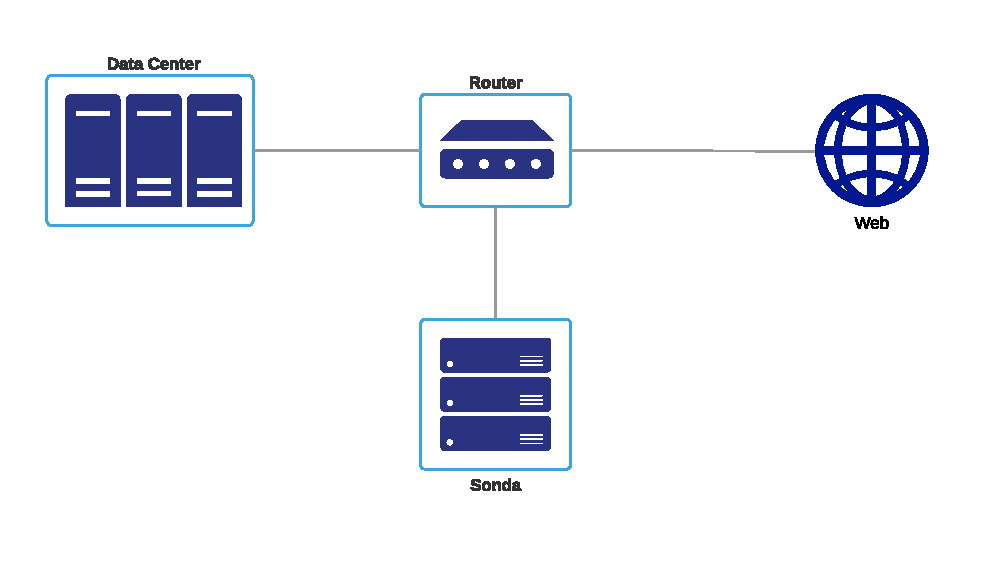
\includegraphics[scale=0.5]{imagenes/arq.pdf} 
		\end{center}
		\end{figure}	
    \item Datos recogidos: RTT, número de conexiones, bps, pps, ...
\end{itemize}
\end{block}
\end{frame}

% DIAPO 2
\begin{frame}
\frametitle{Ejemplos de incidencias}
\begin{block}{Ejemplos de incidencias}


\begin{figure}[ht]
\centering
\subfigure[Ejemplo DDOS]{
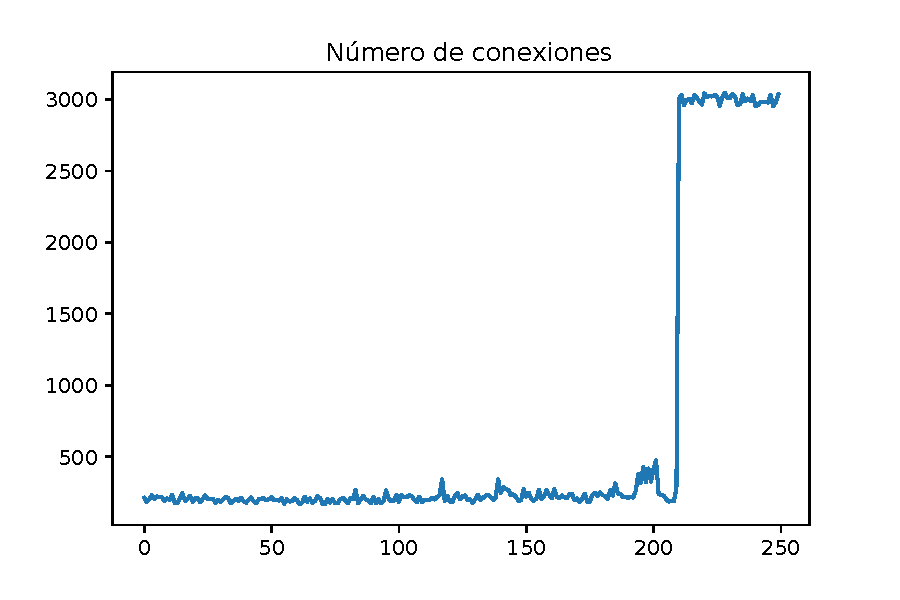
\includegraphics[scale=0.3]{imagenes/ddos.pdf}
}
\qquad
\subfigure[Servicio anómalo]{
    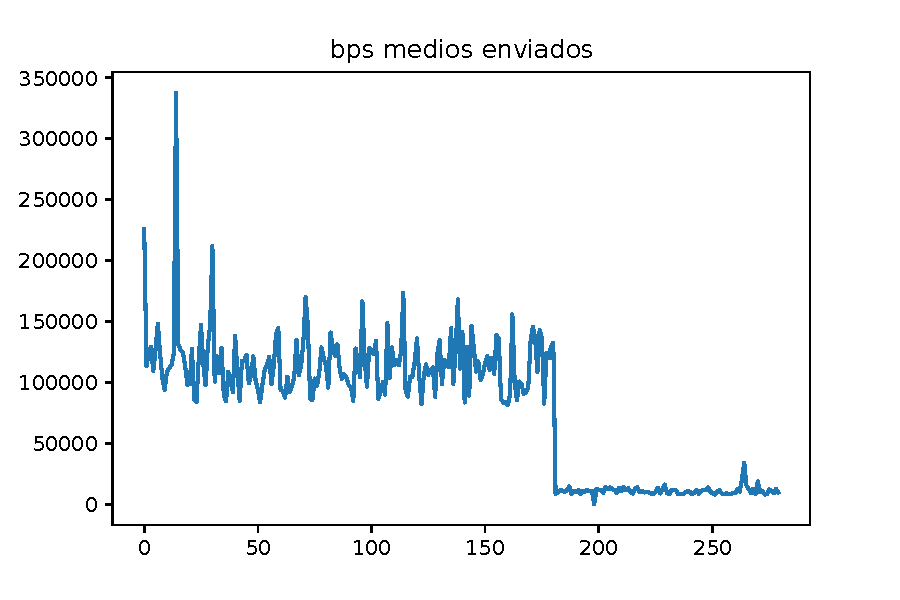
\includegraphics[scale=0.3]{imagenes/server_malfun.pdf}
}
\end{figure}
\end{block}
\end{frame}



% Diapo 3
\begin{frame}
\frametitle{Objetivos}

Diseñar, implementar y evaluar un sistema que:
\begin{itemize}
\item Monitoriza la red.
\item Distingua el comportamiento anómalo del usual.
\item Notifica incidencias.
\end{itemize}

\end{frame}


% Diapo 4
\begin{frame}
\frametitle{Propuesta de modelo}
El modelo se compone de dos partes:
\begin{itemize}
\item Estimación de la serie
\item Clasificación de las métricas
\end{itemize}

\begin{figure}[htb]
\begin{center}
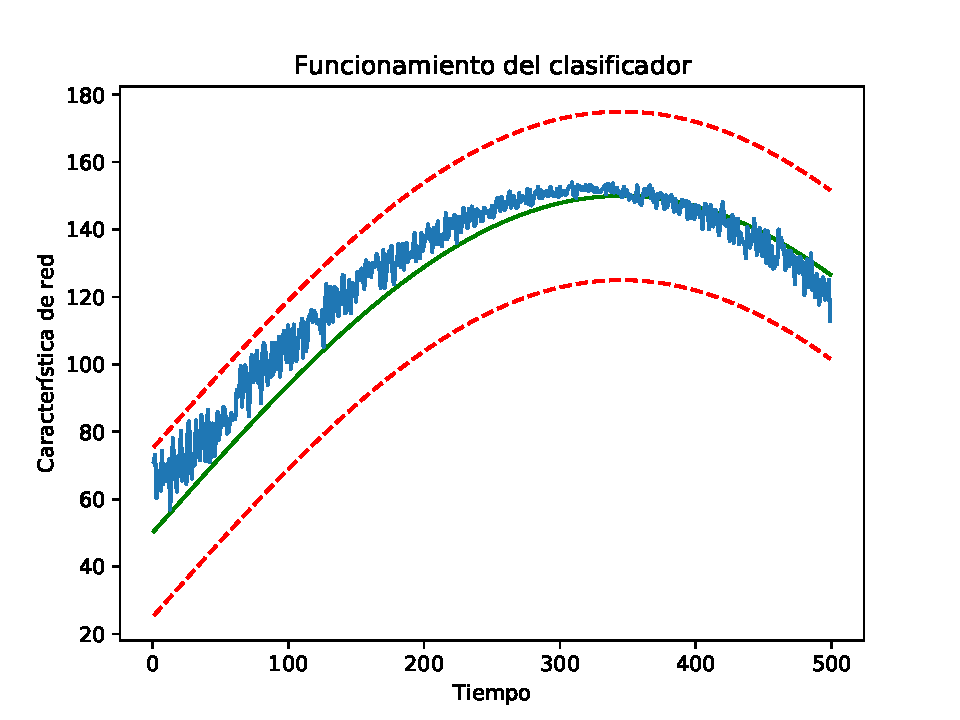
\includegraphics[scale=0.5]{imagenes/funcionamiento.pdf} 
\end{center}
\end{figure}

\end{frame}

% Diapo 5
\begin{frame}
\frametitle{Estimación de la serie}

Regresores utilizados en el modelo:
\begin{itemize}
\item LSTM
\item Auto regresor lineal
\end{itemize}

\begin{figure}[htb]
\begin{center}
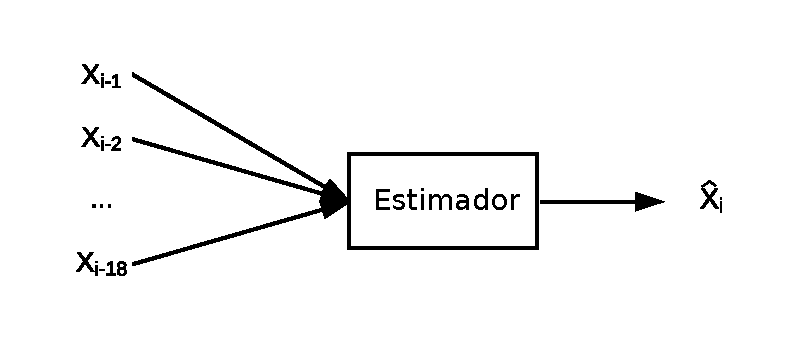
\includegraphics[scale=0.5]{imagenes/estimador.pdf} 
\caption{Esquema de entradas y salidas}
\end{center}
\end{figure}

\end{frame}


% Diapo 6
\begin{frame}
\frametitle{Clasificación}

Se compara $X_i$ con $\hat{X}_i$, si 
\[
\frac{1}{n}|| \hat{X}_i - X_i ||^2 > \mu
\]
se notifica una alarma
 
\end{frame}


% Diapo 7
\begin{frame}
\frametitle{Información adicional}
El modelo no solo identifica anomalías. También aporta:
\begin{itemize}
\item Prioridad de métrica de red:
\[
	r_i^j = \frac{(\hat{X}_i^j - X_i^j)^2}{||\hat{X}_i - X_i ||^2}
\]
\item Prioridad de incidencia:
\[
	p = \frac{\frac{1}{n}||\hat{X}_i - X_i||^2}{\mu}
\]
\end{itemize}
\end{frame}



% Diapo 8
\begin{frame}
\frametitle{\textit{Dataset} de pruebas}

Se probó el modelo con un \textit{dataset} recogido en un centro de datos de una gran empresa de hidrocarburos.
\begin{itemize}
\item Asumimos datos sin incidencias.
\item Simulamos las incidencias para evaluar el modelo.
\end{itemize}
\end{frame}

% Diapo 9
\begin{frame}
\frametitle{Experimento 1}
\begin{block}{Procedimiento}
\begin{itemize}
\item Se entrena con el 70\% sin incidencias.
\item Se inducen diferentes incidencias (5) en el 30\% restante.
\item Se calcula el $F_2$\textit{-score} para un rango de umbrales.
\end{itemize}
\end{block}
\end{frame}


% Diapo 10
\begin{frame}
\frametitle{Resultados del experimento 1}
Resultados para el paquete de incidencias mixto:
\begin{table}{}
	\begin{center}
		\begin{tabular}{ | c || c | c | c | c |  }
			\hline
			Estimador & Umbral & $ F_2 $ & Precisión & Sensibilidad \\
			\hline
			LSTM & 30 & 0.8532 & 90.07\% & 84.21\% \\
			VAR & 18 & 0.9717 & 87.3\% & 100.0\% \\
			\hline
		\end{tabular}
	\end{center}
\end{table}

\begin{itemize}
\item Resultados satisfactorios en algunos servidores de alta agregación.
\item Test para determinar los umbrales
\item Test para determinar eficacia de la clasificación (LSTM vs VAR)
\end{itemize}

\end{frame}

% Diapo 11
\begin{frame}
\frametitle{Experimento 2}

\begin{block}{Procedimiento}
Puesta a prueba en 15 días de datos sin incidencias para evaluar el número de alarmas en circunstancias reales. 

Además, realizamos inspección manual de algunas alarmas para estimar la precisión aparente (que no la sensibilidad).
\end{block}
\end{frame}
 

% Diapo 12
\begin{frame}
\frametitle{Resultados del experimento 2}
Se obtuvo de media por día por servidor:
\begin{itemize}
\item 0.7 alarmas para LSTM.
\item 0.75 alarmas para VAR.
\end{itemize}

\begin{block}{Inspección manual de incidencias}
\begin{figure}
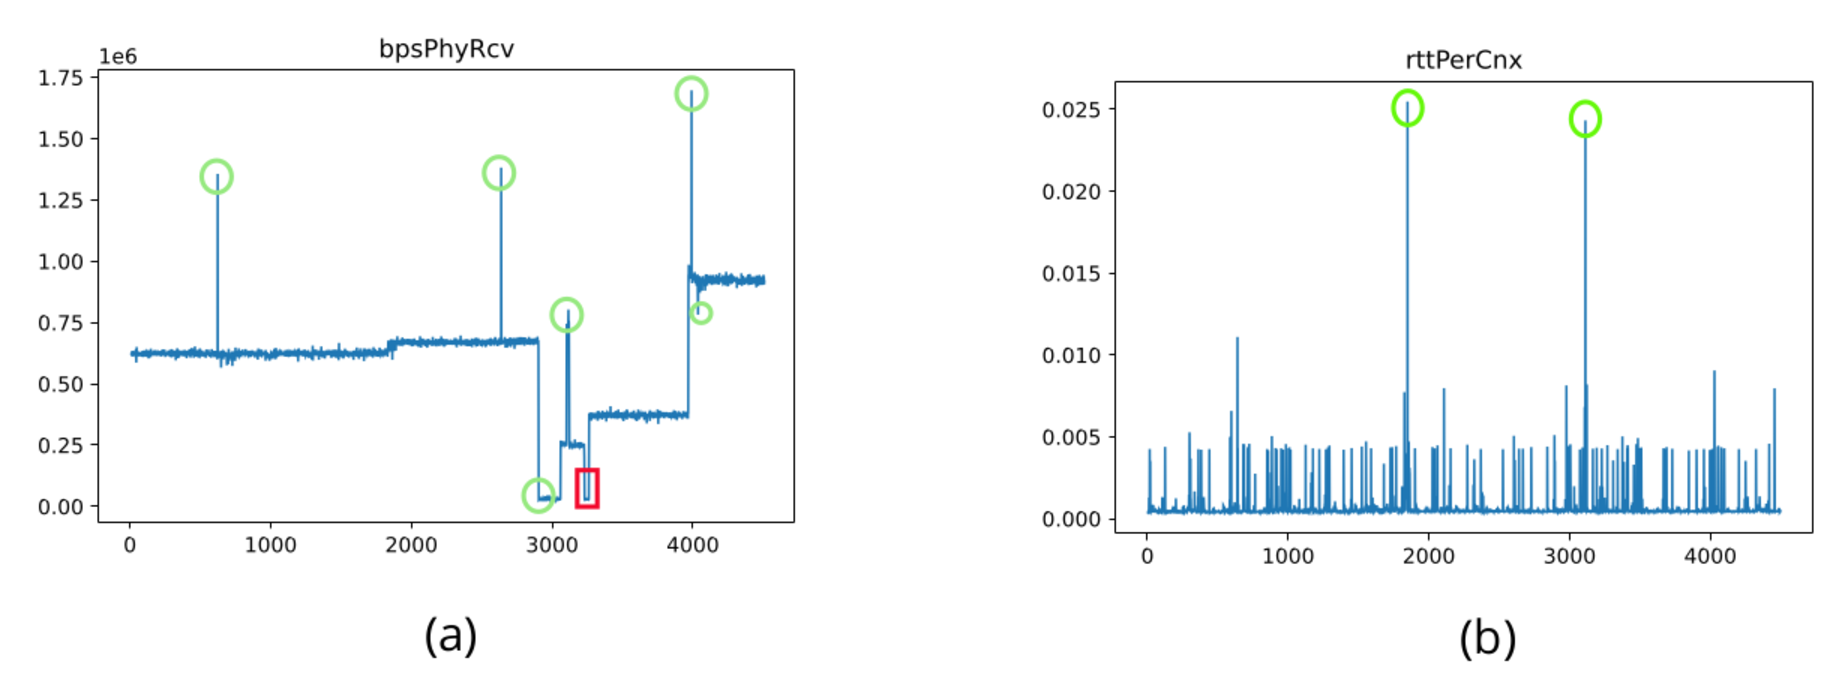
\includegraphics[scale=0.3]{imagenes/manual.pdf} 
\end{figure}
\end{block}
Recordemos la prioridad de incidencias.
\end{frame}


% Diapo 13
\begin{frame}

\frametitle{Conclusiones y trabajo futuro}
\begin{itemize}
\item Es viable la detección automatizada de incidencias.
\item Se pueden proponer alternativas para determinar automáticamente los umbrales de los modelos (descomposición de series).
\item Posible retroalimentación de un gestor en un sistema real para mejorar el modelo.
\end{itemize}

\end{frame}

\end{document}




